\section{Exploratory preprocessing experiments for RQ2}
\label{app:rq2-pilot}

\subsection{Provenance and purpose}
The initial baseline, N47 probes and letter-balanced pilot were implemented and executed by the Codex assistant using the local Kaggle ASL Alphabet images. The student subsequently reported executing the three-stage workflow. The completed \texttt{test\_110} exports support the reproduction documented at the end of this appendix. Program outputs establish the recorded outcomes; operator identity is based on the student's report. Visual assessment remains outstanding.

RQ2 concerns recovery of visually plausible hand landmarks among initially missed images. The measurements below establish technical recovery. The visual plausibility of all recovered configurations has yet to be assessed using a fixed rubric. N47 and other inspected pilot images should be identified as development data when constructing a subsequent evaluation set.

\subsection{Fresh baseline and training}
The baseline processed 78,000 original A--Z training images, comprising 3,000 images per letter. The additional classes were excluded. MediaPipe Hand Landmarker 0.10.35 ran in IMAGE mode, with a maximum of two hands and detection and presence thresholds both set to 0.50. The model file was \texttt{models/hand\_landmarker.task}. A result received \texttt{ok} when exactly one hand was returned and the project's geometric validation passed.

\begin{table}[ht]\centering
\caption{Fresh detection outcomes on original A--Z training images.}
\label{tab:rq2-baseline}
\begin{tabular}{lrr}\toprule
Outcome & Images & Percentage\\\midrule
One valid hand (\texttt{ok}) & 60,251 & 77.245\\
Zero hands (\texttt{no\_hand}) & 17,598 & 22.562\\
Multiple hands & 151 & 0.194\\
Invalid geometry & 0 & 0.000\\\midrule
Total & 78,000 & 100.000\\\bottomrule
\end{tabular}
\end{table}

A fresh SVM letter classifier was fitted to the 60,251 accepted images using 820 Shin descriptors and 15 angle features. This produced \texttt{runs/clean\_training/asl\_clean.joblib}. Its fit has no independent test score. The recovery experiments below use the pretrained MediaPipe detector; the letter classifier does not determine whether a hand is detected.

\subsection{N47 development example}
The original N47 image returned \texttt{no\_hand}. One application of dilation with a square \(3\times3\) kernel changed its output to \texttt{ok} at the same detector thresholds. Erosion and the tested Canny overlay retained \texttt{no\_hand}. In separate threshold probes on the original pixels, lowering only the detection threshold to 0.49 retained \texttt{no\_hand}, while 0.45 yielded \texttt{ok}. These probes show sensitivity to both preprocessing and threshold choice.

The initial N47 probes were executed as terminal commands, and their outputs were recorded in the conversation. They were not exported as a dedicated CSV. The original-versus-dilation transition was subsequently rerun when generating the example images below. The exact internal detection score was not recorded.

\begin{figure}[ht]\centering
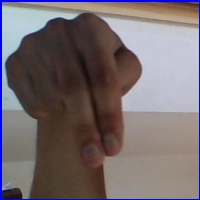
\includegraphics[height=30mm]{rq2_examples/N47_original.png}\hspace{8mm}
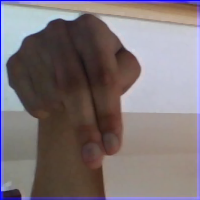
\includegraphics[height=30mm]{rq2_examples/N47_dilated.png}\hspace{8mm}
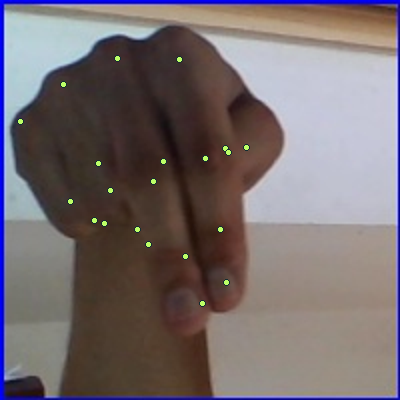
\includegraphics[height=30mm]{rq2_examples/N47_overlay.png}
\caption{N47 in its original form (left), after dilation (centre), and with recovered points overlaid on the original pixels (right). The overlay supports inspection; it does not constitute an independent landmark accuracy assessment.}
\label{fig:rq2-n47}
\end{figure}

\clearpage
\subsection{Letter-balanced pilot}
Using random seed 42, the pilot selected 20 initially missed and 10 initially accepted images per letter, giving 520 misses and 260 controls. The original status was rechecked before applying each transformation. Every selected photo received each of the three transformations below, with fixed detector settings.

\begin{itemize}
\item Dilation used \texttt{cv2.dilate} with a \(3\times3\) square kernel and one iteration.
\item Erosion used \texttt{cv2.erode} with the same kernel and iteration count.
\item The Canny overlay used a grayscale conversion, a \(5\times5\) Gaussian blur and Canny thresholds of 50 and 150. The three-channel edge map was added to the original RGB image with weights 0.25 and 1.0, respectively.
\end{itemize}

Image dimensions were retained, and processed arrays were supplied directly to the detector. Technical recovery means a transition from \texttt{no\_hand} to \texttt{ok}. Control loss means that an originally accepted image no longer received \texttt{ok}.

\begin{table}[ht]\centering
\caption{Exploratory pilot outcomes. Recovery denominators are 520 misses; loss denominators are 260 controls.}
\label{tab:rq2-pilot}
\begin{tabular}{lrrrr}\toprule
Transformation & Recovered & Recovery (\%) & Control losses & Loss (\%)\\\midrule
Dilation & 130 & 25.00 & 6 & 2.31\\
Erosion & 64 & 12.31 & 8 & 3.08\\
Canny overlay & 49 & 9.42 & 28 & 10.77\\\bottomrule
\end{tabular}
\end{table}

The pilot gave equal weight to each letter, whereas the complete set of missed images has unequal letter counts. Its recovery percentage therefore does not directly estimate recovery across all 17,598 misses. Control losses describe applying preprocessing to already accepted images. A second-attempt procedure restricted to baseline misses bypasses these controls.

\subsection{Code and retained evidence}
All paths below are relative to the project root containing \texttt{app.py}.
\begin{itemize}
\item \texttt{research/data.py}, class \texttt{Detector}, defines detector settings and geometric validation.
\item \texttt{research/clean\_training.py} runs the baseline and prepares accepted inputs. The fresh classifier fit uses \texttt{--fresh-fit} in \texttt{research/live\_model.py}.
\item \texttt{research/morphology\_pilot.py} contains the transformations, deterministic sampling, paired comparisons and pilot exports.
\item \texttt{runs/clean\_training/all\_images.csv}, \texttt{no\_hand.csv} and \texttt{by\_letter.csv} contain the baseline inventory and summaries.
\item The pilot directory is \texttt{runs/clean\_training/morphology\_pilot/}. It contains \texttt{per\_foto.csv} with paired outcomes, \texttt{summary.csv} with aggregate results and \texttt{controle\_*.jpg} with overlays of recovered detections.
\end{itemize}

The original pilot exports status changes and rendered overlays. The subsequent three-stage workflow also exports landmark coordinates in \texttt{retry\_landmarks.jsonl}. A completed visual-review dataset remains outstanding. The earlier \texttt{historical\_image\_audit.py} reconstructed historical cohort membership. The fresh detector outputs listed above support the present baseline counts.

\subsection{Reproduction and next measurement}
Run \texttt{python -m research.clean\_training --out runs/clean\_training}
from the project root with the configured Python environment. The command requires a new output directory. The existing baseline can be used to rerun \texttt{python -m research.morphology\_pilot}; this command writes to the existing pilot output paths. Preserve the original evidence before rerunning it.

\clearpage
\subsection{Student-reported reproduction and program evidence}
\label{app:rq2-reproduction}
The completed run is \path{experiments/hand_detection_recovery/runs/test_110}.
It used \texttt{--limit 110}, selecting A1--A110 in dataset order. This is a technical reproduction on a single letter. It contains no N47 image and does not estimate recovery across A--Z.
The preserved evidence is located at \path{paper/evidence/rq2_test_110}.
The following tables were checked against the paired rows and landmark exports, in addition to the program summary.

\begin{table}[ht]\centering
\caption{Recomputed outcomes for \texttt{test\_110}. Recovery rates use 46 baseline misses as the denominator.}
\begin{tabular}{lrr}\toprule
Quantity & Count & Percentage\\\midrule
Original images & 110 & 100.00\\
Originally accepted & 64 & 58.18\\
Initially missed & 46 & 41.82\\\midrule
Recovered by dilation & 6 & 13.04\\
Recovered by erosion & 2 & 4.35\\
Recovered by Canny overlay & 0 & 0.00\\
Recovered by at least one variant & 8 & 17.39\\\bottomrule
\end{tabular}
\end{table}

Counting each image once, original acceptance plus any technically successful retry gives \(72/110=65.45\%\) coverage, compared with \(64/110=58.18\%\) initially. The increase is 7.27 percentage points. This combined outcome allows any of the three variants to succeed.

\begin{table}[ht]\centering
\caption{Recovered images from \texttt{per\_image.csv}. All originally had status \texttt{no\_hand}.}
\begin{tabular}{ll}\toprule
Successful variant & Original filenames\\\midrule
Dilation & A59.jpg, A74.jpg, A75.jpg, A90.jpg, A92.jpg, A98.jpg\\
Erosion & A85.jpg, A89.jpg\\\bottomrule
\end{tabular}
\end{table}

\paragraph{Evidence traceability.}
\texttt{baseline.csv} records original detections. \texttt{no\_hand.csv} identifies the 46 candidates.
\texttt{processed.csv} maps their 138 variant images to original IDs and records image checksums.
\texttt{per\_image.csv} supplies paired statuses and successful variants.
\texttt{summary.csv} gives aggregate counts, while \texttt{unrecovered.csv} identifies the 38 remaining misses.
\texttt{retry\_landmarks.jsonl} contains the retry outputs and recovered coordinates.
\texttt{settings.json} records MediaPipe 0.10.35, OpenCV 4.14.0, filter parameters, detector settings and code/model hashes.
The archive's \texttt{evidence\_manifest.json} records SHA256 checksums of these exports.
Absolute image paths refer to the original workstation; the PNGs remain in the source run.

\paragraph{Reproduction.}
Use the project's configured Python environment from the root containing \texttt{app.py}.
The following command invokes the existing baseline, preprocessing and retry functions in sequence:
\begin{verbatim}
python experiments/hand_detection_recovery/run.py --name test_110 --limit 110
\end{verbatim}
The wrapper starts clean and deletes existing outputs with that run name. Use a new name to preserve a live run, or add \texttt{--resume} to continue it. The separate evidence archive survives cleaning the run folder.

\paragraph{Verification of exported results.}
The read-only check below recomputes recovery counts and percentages, checks image-ID and variant correspondence, and confirms that accepted retry records contain one hand with 21 image landmarks.
\begin{verbatim}
python experiments/hand_detection_recovery/verify_results.py \
  --run paper/evidence/rq2_test_110
\end{verbatim}
Enter this as one line in PowerShell, omitting the displayed backslash.
Verification passed for the archived exports. This establishes internal consistency of the recorded measurements. Visual landmark quality and the final dataset-wide recovery result remain to be evaluated. At inspection, \texttt{full\_dataset\_01} contained partial progress but no completed result summary.

